\chapter{Specifikace požadavků}

\indent

Zadání vzniklo původně z požadavku na rozšíření mobilní aplikace Catcher, ke které se ještě
dostaneme v analýze již fungujících řešení. Se vznikajícími nároky na rozšiřitelnost přišel
také požadavek na rozhraní, které by backend obsluhovalo. Mým řešením je samostatná webová
služba, kterou bude využívát libovolný klient, např. webová aplikace Jaroslava Veselého. 

\section{Požadavky na Catchera}

\indent

Na základě diskuse s ČALD, častými organizátory turnajů a některými hráči byly stanoveny
funkční a nefunkční požadavky na vznikající aplikaci.

\subsection{Funkční požadavky}

\subsubsection*{Import a export dat}
Systém umožňuje import oddílů a jeho hráčů z databáze ČALD.

\subsubsection*{Rozpis zápasů}
Oprávněná role může vytvořit svůj vlastní turnaj a vložit seznam všech zápasů,
které se budou hrát. Vytvořený rozpis zápasů systém již doplňuje automaticky na základě
odehraných výsledků (např. vítěze semifinále automaticky posune do finále). Ve chvíli,
kdy to bude již možné, doplní celkové pořadí turnaje. Automatické doplnění se týká i 
souhrné tabulky vzájemných hodnocení v kategorii SOTG.

\subsubsection*{Zadávání dat v rámci turnaje}
Každý tým má možnost vytvořit vlastní soupisku na turnaj, kde bude hrát. Systém pak umožňuje
v průbehu turnaje zadávat konkrétní údaje:
\begin{itemize}
  \item průběžné skóre zápasů nebo jejich závěrečný výsledek
  \item skórující a asistující hráč
  \item hodnocení SOTG
\end{itemize}

\subsubsection*{Tvorba statistik}
Systém tvoří detailní statistiky hráčů, týmů a zápasů (obdržené a udělené body,
počet asistencí, průměrná hodnota SOTG).

\subsection{Nefunkční požadavky}

\subsubsection*{Snadná rozšířitelnost}
Už nyní evidujeme změny, o které je zájem, ale nejsou předmětem této práce.
I proto je nutné projekt dokončit tak, aby byl v budoucnu snadno rozšiřitelný nebo
modifikovatelný.

\subsubsection*{Nízká cena}
Cílem není vytvořit výdělečný projekt, ale fungující službu pro několik stovek hráčů
a fanoušku v České republice. I proto je požadavkem použití volně dostupných
knihoven a technologií.

\subsubsection*{Výkon}
Podle celkem jednoduchých odhadů lze usoudit, že aplikaci budou čekat výkyvy v provozu.
Většina zápisů a čtění dat probíhá během samotných turnajů. Podle statistických údajů
z již užívané aplikace Catcher víme, že během špičky není počet požadavků za sekundu
větší než několik desítek. I proto není na celkový výkon kladen žádný zvláštní požadavek.
Systém by každopádně měl více jak 95 \% žádostí zpracovat do jedné vteřiny a na žádnou z nich
nedpovědět za více jak 5 sekund.

\subsubsection*{Spolehlivost}
Spolehlivost je základem pro funkční běh Catchera. Velká část operací, včetně chybných budou
zapisovány do souborů pro snadné odhalení chyb. Obnova musí být proveditelná ze zálohovacích souborů.
%V případě výpadku by měl být informován administrátor pomocí SMS nebo emailu.

\subsubsection*{Bezpečnost}
% TODO: IDEA: popsat nejak autentizaci a autorizaci
Systém musí jednoznačně určit a ověřit uživatele, který přistupuje k rozhraní Catchera. Zároveň
musí existovat možnost za chodu přidávat, odebírat nebo měnit oprávnění. Dále pak systém musí
být datově integritní, tzn. že obsah zpráv nebude při přenosu změněn. Pro tento projekt není
nutné používat HTTPS protokol.

\subsubsection*{Nároky na hardware}
Systém musí být schopen běžet na běžných serverech s ne více jak 4GB RAM.

\subsubsection*{Formát importu}
Pro import soupisek musí systém umět číst data ve formátu, který ČALD pro export používá.

\subsubsection*{Vytvoření dokumentace}
Pro potřeby vývoje frontendu je potřeba vytvořit dostatečně detailní dokumentaci rozhraní API.

\section{Uživatelské role}

\subsubsection*{Nepřihlášený návštěvník}

Jde o nejčastější přístup k aplikaci. Slouží k zobrazení všech statistik (aktuální skóre,
statistika všech hráčů, hodnocení SOTG). Nemůže žádná data vytvářet nebo modifikovat
a nevyžaduje přihlášení.
  
\subsubsection*{Organizátor}

Účet pod touto rolí může vytvořit kdokoliv pouhou registrací. Po příhlášení lze přídávat
nové turnaje a ty následně editovat. Tím se rozumí tvorba rozpisu zápasů a seznamu účastníků
z již existujícího seznamu týmů. Dále může zadávat průběžné a výsledné skóre zápasů,
skórující a asistující hráče a vidí na tabulku vzájemných hodnocení SOTG pro účely vyhlášení
vítěze. Tato tabulka je pro ostatní role až do vyhlášení nezobrazitelná.

\subsubsection*{Klubový/oddílový účet}

Pro účely odevzdávání hodnocení SOTG a úprav v týmové soupisce je vytvořen pro každý oddíl
jeden společný účet. Tento účet má možnost vytvořit pouze administrátor. Přihlašovací údaje pak
získá zástupce klubu a je pouze na něm, kdo z jeho oddílu bude spravovat vytvořený učet.
Součástí klubu může být více týmů, např. mužský a ženský tým nebo A tým a B tým.
  
\subsubsection*{Administrátor}
Má plnou kontrolu nad správou účtů a nad daty v databázi. Jeho možnosti zahrnují možnosti
všech ostatních rolí.

\section{Případy užití}

Následující část popisuje nejběžnější případy užití. V návrhu rozhraní jde
o jednu z nejdůležitejších součastí, protože určuje směr návrhu. Výsledné API by tak mělo
pokrývat všechny níže uvedené případy. Následující seznam zachycuje jednotlivé požadavky
a jejich popis:

% TODO: Co budou nejbeznejsi operace v aplikaci (zapisovani skore, zapisovani spiritu, tvorba turnaje a rozpisu).
% Tady to mozna napsat VSECHNO v bodech, protoze z toho budou vychazet API.
% TODO: Napsat, kdo vsechno muzes tyto operace delat. Napr. organizator muze ukoncit zapas.

\subsection*{Import}
  \begin{description}
    \item[UC1: Import dat z databáze ČALD] \hfill \\
    Doplňuje seznam oddílů a jejich hráčů do databáze Catchera. Manuálně lze stáhnout
    %V pravidelném intervalu stáhne
    aktuální data z ČALD databáze a doplní doposud aktuální data v databázi.
  \end{description}

\subsection*{Uživatelé}
  \begin{description}
    \item[UC2: Registruje nového uživatele] \hfill \\
    Kdokoliv se může stát organizátorem turnaje. Stačí se zaregistrovat s platným emailem.
    Klubové účty vytváří administrátor.
    \item[UC3: Autentizuje uživatele] \hfill \\
    Určí skutečnou identitu uživatele. Jinými slovy jej přihlásí.
    \item[UC4: Odesílá zapomenuté heslo] \hfill \\
    Pokud má uživatel přístup ke svému emailu, přijde mu nové heslo ke svému účtu.
  \end{description}

\subsection*{Oddíly}
  \begin{description}
    \item[UC5: Vytvoří oddíl] \hfill \\
    Uloží nový oddíl do databáze.
    \item[UC6: Získá oddíly] \hfill \\
    Vrátí informace o jednom nebo více oddílech.
    \item[UC7: Edituje oddíl] \hfill \\
    Upraví informace o oddílu.
    \item[UC8: Smaže oddíl] \hfill \\
    Smaže oddíl z databáze.
  \end{description}

\subsection*{Hráči}
  \begin{description}
    \item[UC9: Vytvoří hráče] \hfill \\
    Klubový účet a administrátor mají možnost vytvořit nového hráče. Hráči lze vytvořit vazba
    pouze k jednomu klubu. Kromě jména a příjmení u něj lze uložit číslo dresu a jeho přezdívku.
    \item[UC10: Získá hráče] \hfill \\
    Vrátí informace o jednom nebo více hráčích.
    \item[UC11: Edituje hráče] \hfill \\
    Klubový účet a administrátor mohou upravovat informace o klubu.
    \item[UC12: Smaže hráče] \hfill \\
    Administrátor může smazat hráče.
  \end{description}

\subsection*{Týmy}
  \begin{description}
    \item[UC13: Vytvoří tým] \hfill \\
    Klubový účet a administrátor má možnost vytvořit tým spadající pod klub. Týmu musí přiřadit
    konkrétní divizi (např. open) a stupeň (např. A~tým).
    \item[UC14: Získá týmy] \hfill \\
    Vrátí informace o jednom nebo více týmech.
    \item[UC15: Edituje tým] \hfill \\
    Klubový účet a administrátor mohou upravovat informace o týmu. 
    \item[UC16: Smaže tým] \hfill \\
    Právem smazat tým disponuje pouze administrátor.
  \end{description}

\subsection*{Turnaje}
  \begin{description}
    \item[UC17: Vytvoří turnaj] \hfill \\
    Organizátor a administrátor vytvoří turnaj. Do databáze se uloží účastníci turnaje,
    základní skupiny, zápasy ve skupinách a play-off.
    \item[UC18: Edituje turnaj] \hfill \\
    Oprávněné role upraví informace o turnaji.
    %Aby se mohly editovat soupisky týmů na turnaji a započítávat výsledky, musí být turnaj aktivovaný příznakem \pythoninline{ready}. 
    \item[UC19: Získá turnaje] \hfill \\
    Vrátí informace o jednom nebo více turnajích.
    \item[UC20: Získá konečné pořadí] \hfill \\
    Získá známé pořadí týmů na turnaji a pokud turnaj již skončil, zobrazí i hodnocení SOTG.
  \end{description}

  \subsubsection*{Týmové soupisky}
    \begin{description}
      \item[UC21: Připsat hráče na soupisku] \hfill \\
      Klub, organizátor nebo administrátor týmu přiřadí hráče, tzn. vytvoří soupisku na turnaj.
      Každý hráč může hrát na turnaji pouze za jeden tým. Hráčům ze soupisky pak lze připisovat body na turnaji.
      \item[UC22: Získá soupisky] \hfill \\
      Vrátí soupisku konkrétního týmu nebo seznam hráčů napříč celým turnajem. Včetně jejich statistik.
      \item[UC23: Odebere hráče ze soupisky] \hfill \\
      Jestliže hráč nedisponuje žádnými statistikami a je zřejmé, že do žádného zápasu nezasáhl, je možné jej odstranit ze soupisky.
    \end{description}
  
  \subsubsection*{Skupiny a zápasy}
    \begin{description}
      \item[UC24: Získá skupiny] \hfill \\
      Vrátí informace o vybraných skupinách. Seznam týmů včetně jejich vzájemného skóre a pořadí ve skupině.
      \item[UC25: Získá zápasy] \hfill \\
      Vrátí stav, výsledné skóre, nebo hodnocení SOTG vybraných zápasů.
      \item[UC26: Upraví zápas] \hfill \\
      Zahájit nebo ukončit zápas může organizátor a administrátor. Dále lze změnit hřiště, na kterém se bude hrát nebo výsledné skóre.
      \item[UC27: Vytvoří nový bod v zápase] \hfill \\
      Každý bod, který se odehraje, může evidovat skórujícího, nahrávajícího hráče a informaci, zda šlo o Callahan
      \footnote{Callahan je speciální bod, při kterém skórujícímu hráči létající talíř nahraje soupěř.}. Data může vkládat pouze organizátor nebo administrátor.
      \item[UC28: Smaže body v zápase] \hfill \\
      V případě potřeby může organizátor nebo administrátor smazat vložené body.
    \end{description}
    
  \subsubsection*{SOTG na turnaji}
    \begin{description}
      \item[UC29: Ohodnotí soupeře v daném zápase hodnocením SOTG ] \hfill \\
      Po každém zápase může uživatel z klubového účtu ohodnotit soupeře hodnocením SOTG. Toto hodnocení se skládá...
      \item[UC30: Upraví již jednou odevzdané hodnocení SOTG ] \hfill \\
      Při potřebě změnit hodnocení jej lze ještě před oficiálním ukončení turnaje upravit.
      \item[UC31: Získá všechna odevzdaná hodnocení SOTG] \hfill \\
      Do ukončení turnaje viditelné pouze pro organizátora.
      \item[UC32: Získá všechna neodevzdaná hodnocení SOTG] \hfill \\
      Před ukončením turnaje lze zkontrolovat, zda jsou všechna hodnocení již odevzdaná.
      V opačném případě zobrazí seznam týmů, které hodnocení neodevzdaly.
    \end{description}
    
    
\begin{figure}[ht!]
\centering
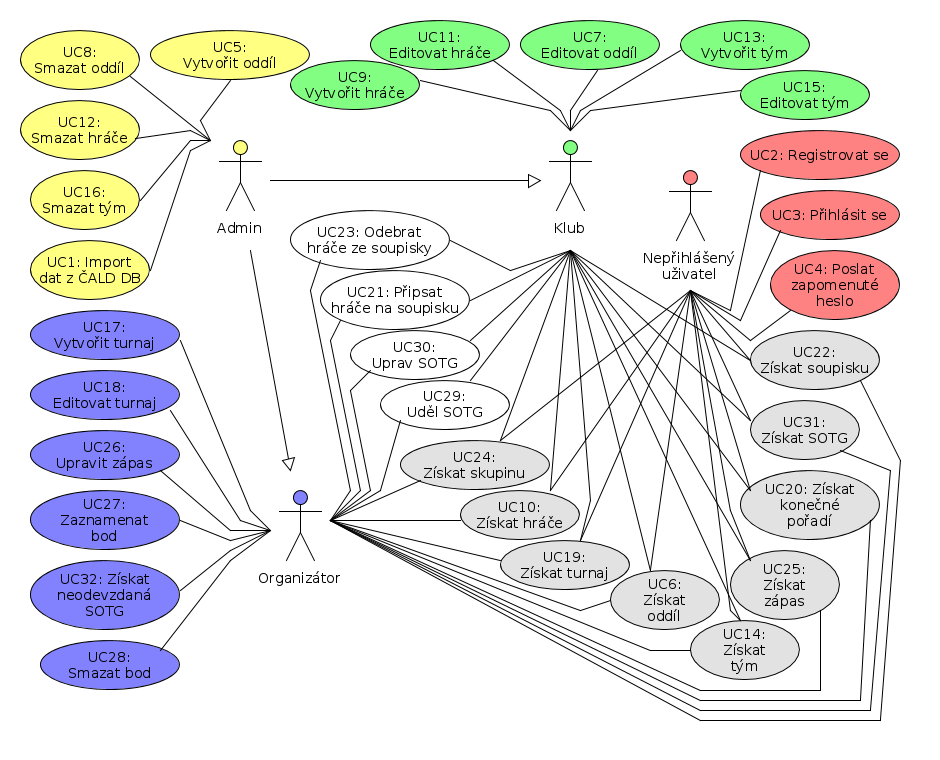
\includegraphics[width=130mm]{./images/use-case.png}
\caption{Use case diagram\label{overflow}}
\end{figure}
    
% \begin{description}
% 
% \item[Získání libovolného turnaje z databáze] \hfill \\
% Získá množinu turnajů, jež jsou v databázi uloženy. S pomocí několika parametrů lze tuto
% množinu filtrovat:
% \begin{itemize}
%    \item turnaj s konkrétním identifikátorem
%    \item pouze ne/ukončené turnaje
%    \item pouze ne/aktivní turnaje
%    \item turnaje odehrávající se v čase od do
%    \item turnaje v kategoriích open, women, mix apod.
%    \item turnaje vytvořené konkrétním uživatelem
%  \end{itemize}
%  Prvek množiny obsahuje informace o turnaji, jako například název, popis, termín a místo turnaje.
%
% \item[Získá účastníky turnaje] \hfill \\
% Ke konkrétnímu turnaji získá kolekci všech týmů, jež se účastní. 
% 
% \item[Získá týmovou soupisku] \hfill \\
% Ke konkrétnímu týmu získá kolekci všech hráčů, jenž se účastní.
% 
%\item[Zadání skórujícího nebo asistujícího hráče] \hfill \\
% V průběhu zápasu umožňuje zadat skórujícího nebo asistujícího hráče.
% 
%\item[Ukončit zápas s výsledným skóre] \hfill \\
% Ukončí zápas a uloží jeho výsledek do databáze.
% 
% \item[Zadat hodnocení SOTG] \hfill \\
% Po ukončení zápasu lze z týmového účtu udělit soupeři hodnocení SOTG. Tento údaj se uloží do tabulky, kde jsou všechna vzájemná hodnocení. 
% 
% \item[Zobrazit tabulku vzájemných hodnocení SOTG] \hfill \\
% Odešle uživateli vhodnou strukturu, kde budou jasně uvedeny všechna doposud vyplněná hodnocení kategorie SOTG.
% 
% \item[Zobrazit pořadí týmů v kategorii SOTG] \hfill \\
% Vrátí pořadí týmů v kategorii SOTG, včetně průměru všech obdržených hodnocení, a informaci o tom, zda je toto pořadí již finální.
% 
% \item[Ukončit turnaj] \hfill \\
% Změní stav turnaje na ukončený. Tabulka vzájemných hodnocení SOTG a výsledné pořadí se tím stanou veřejnými. 
% 
% \item[Zobrazit výsledky všech zápasů] \hfill \\
% 
% \item[Zobrazit detail konkrétního zápasu] \hfill \\ hráči, body, čas
% 
% \item[Získá seřazené hráče podle bodování] \hfill \\ Seřadí hráče na základě bodovaní.
%\end{description}